\documentclass[twocolumn,10]{article}
\newgeometry{top=1cm, bottom=1cm}
\usepackage{hyperref}

\usepackage{graphicx}  % needed for figures
\usepackage{dcolumn}   % needed for some tables
\usepackage{bm}        % for math
\usepackage{amssymb}   % for math
\usepackage{amsmath}
\usepackage{nameref}
\newcommand{\degree}{\ensuremath{^\circ}}
\def\mean#1{\left< #1 \right>}
%%% make INLINE SUBSECTIONS 
	
	% 1em is in the 'sep' slot, which controls how much space is between the numbering and the section heading text. 1em is equal to the width of 1 times the width of a capital 'M' in font you're using. 
\usepackage{titlesec}
\titleformat{\subsection}[runin]
{\normalfont\large\bfseries}{\thesubsection}{1em}{}
	% The formatting settings above other than the 'runin' option are the default settings for subsections. 


\begin{document}
\title{Problem set }
\author{Giulio Ungaretti}
\date{\today}
\twocolumn[
   \begin{@twocolumnfalse}
     \maketitle
     \begin{abstract}
       Problem set solutions.
     \end{abstract}
     \tableofcontents
   \end{@twocolumnfalse}
  ]

\clearpage
\section{Distributions \& \\ probabilities} % (fold)
	\label{sec:Distributions and probabilities}
	\subsection{} % (fold)
	\label{sub:}
	% subsection  (end)
	Given the PDF:
	\begin{equation}
		\operatorname{f}{\left (t \right )} = C e^{- \frac{t}{\tau}}
	\end{equation}
	in the range $t$ $\in~$[$ t_0, \infty $], the value of C for which the PDF is normalized is:

	\begin{equation}
		\int_{t_{{0}}}^{\infty} C e^{- \frac{t}{\tau}}\, dt = 1 \longrightarrow C =  \frac{
		e^{
		\frac{t_0}{\tau}
		}}
		{\tau}
	\end{equation}
	I note a close resemblance of our PDF to the exponential distribution, and they coincide if $t_0 = 0$. 
	The mean or better the expectation  value is then:
	\begin{equation}
	\mathbb{E} [t] = \int_{t_0}^{\infty} t \operatorname{f}{(t) d t } \longrightarrow  t_0 + \tau
	\end{equation}
	It's nice to note that $t_0 = 0$ it matches the well known result for the exponential distribution.
	The width could be quantified with the variance as:
	\begin{multline}
		Var(t) = \mathbb{E}[x^2] - (\mathbb{E}[x])^2 = \\
		= 
		\int_{t_0}^{\infty} t^2 \operatorname{f}{(t) d t } 
		-(\int_{t_0}^{\infty} t \operatorname{f}{(t) d t })^2 = \\
		= 2 \tau ^ 2 - 2 t_o \tau +t_0 ^2  - ( t_0 + \tau ) ^ 2 = \\
		= \tau ^ 2 - 4 \tau t_0 
	\end{multline}
	and once more if $t_0 = 0 $ the variance of the starting PDF coincides withe the one of the exponential distribution. 
	\begin{figure}[htb]
		\begin{center}
			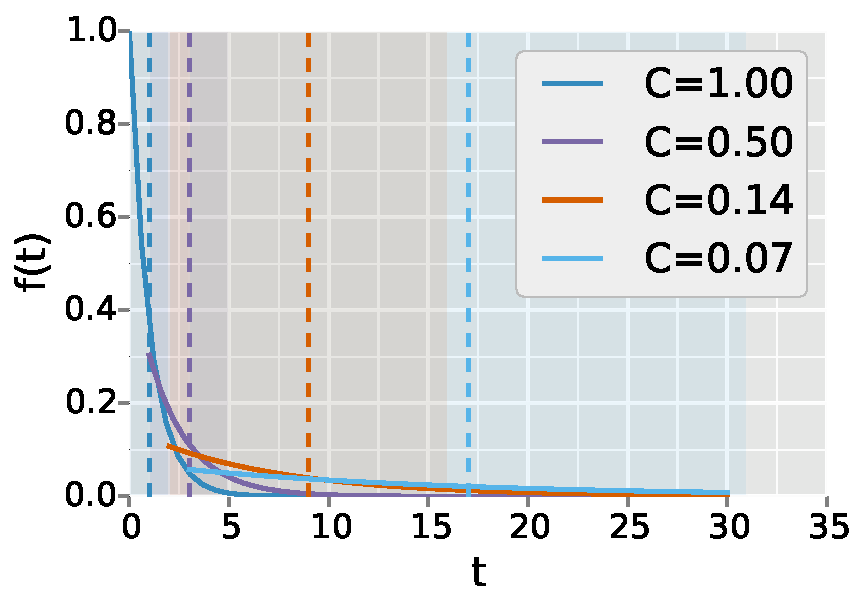
\includegraphics[width= 0.4 \textwidth]{fig/graph.pdf}
		\end{center}
		\caption{Plot of the given PDF, for different values of $ \tau $ and $t_0 $. Dashed lines are the calculated expectation values, and the shaded area represent $\pm$ one square root of the variance around the mean.}
		\label{fig:pdf}
	\end{figure}
	A graphical representation of all said above is found in Figure~\ref{fig:pdf}.
	\subsection{} % (fold)
	\label{sub:}
	Assuming that little Peter is a fair pal, and is using fair coins then the probability of success (heads) follows the binomial distribution.
	If we call $n$ the number of tries, $p= \frac{1}{2}$ the probability for each event to success, and $r$ the number of success out of $n$ tries:
	\begin{multline}
	\label{eq:bin}
		P (n,r) = \frac{n!}{r!(n-r)!} p ^ r (1-p)^{n-r} \\ 
		 = \tbinom n r p ^ r (1-p)^{n-r}
	\end{multline}
	The \emph{chance} of getting 14 or more heads with 20 coin flips is low. As it is possible to see in Figure~\ref{fig:lil}. The probability of getting 14 heads is $\approx 0.036$, and by integrating equation \ref{eq:bin} from r=14 to infinity it is possible to quantify the aforementioned low chance.
	\begin{figure}[h]
		\begin{center}
			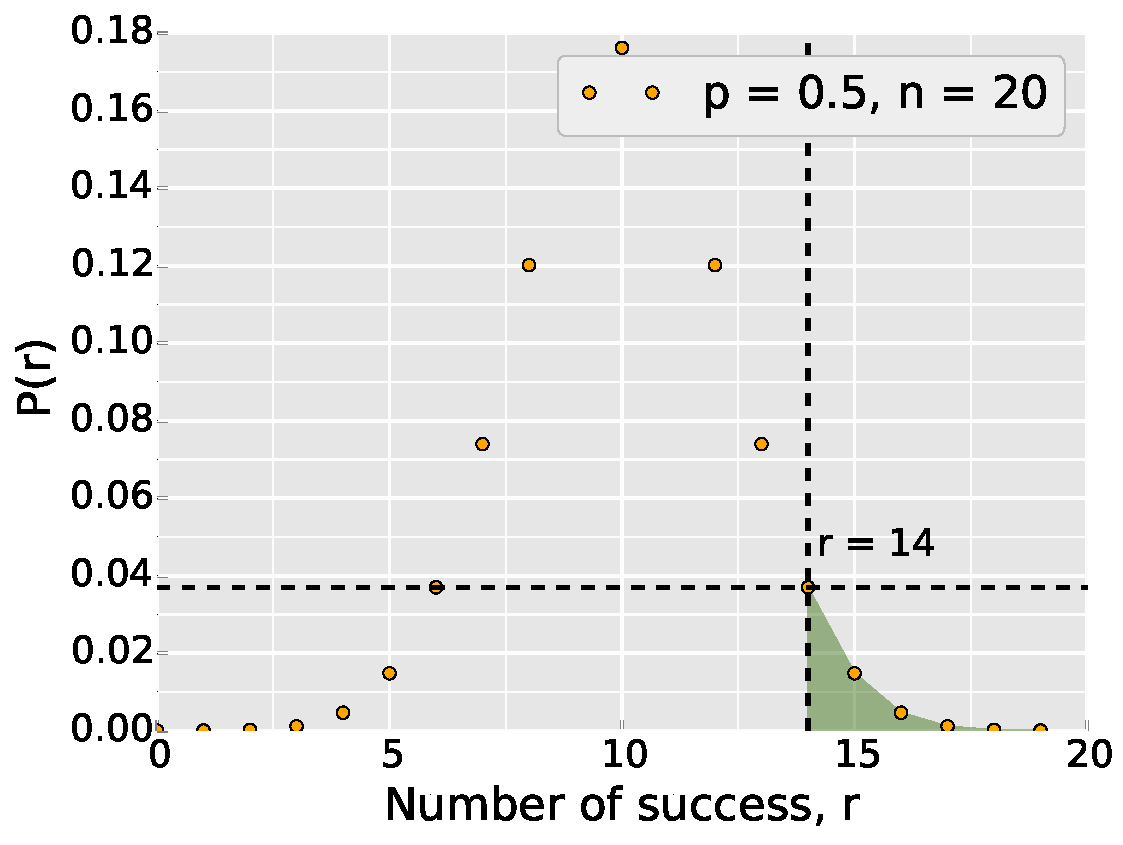
\includegraphics[width=.4\textwidth]{fig/lil.pdf}
		\end{center}
		\caption{Probability of coin flips. The parameters are reported in the legend, and the shadowed area quantifies the chance of getting 14 or more heads.}
		\label{fig:lil}
	\end{figure}


	To find the chance that little Peter gets at least 18 coin at once when flipping 20 coins 100 times, first the probability $P_{18}$ is calculated with equation \ref{eq:bin} using $p= \frac{1}{2}$, $n=20$, and $r=18$.
	It is easy to see that the distribution of the chances of getting at least 18 successes is still binomial but with p = $P_{18}$, $n=100$, and $r=1$.
	The probability of getting one time a success is: $P(1) \approx 0.0177$. The chance of getting more than one is quantified as said before and it is rapresenented as the shaded area in Figure~\ref{fig:lil2}

	\begin{figure}[h]
		\begin{center}
			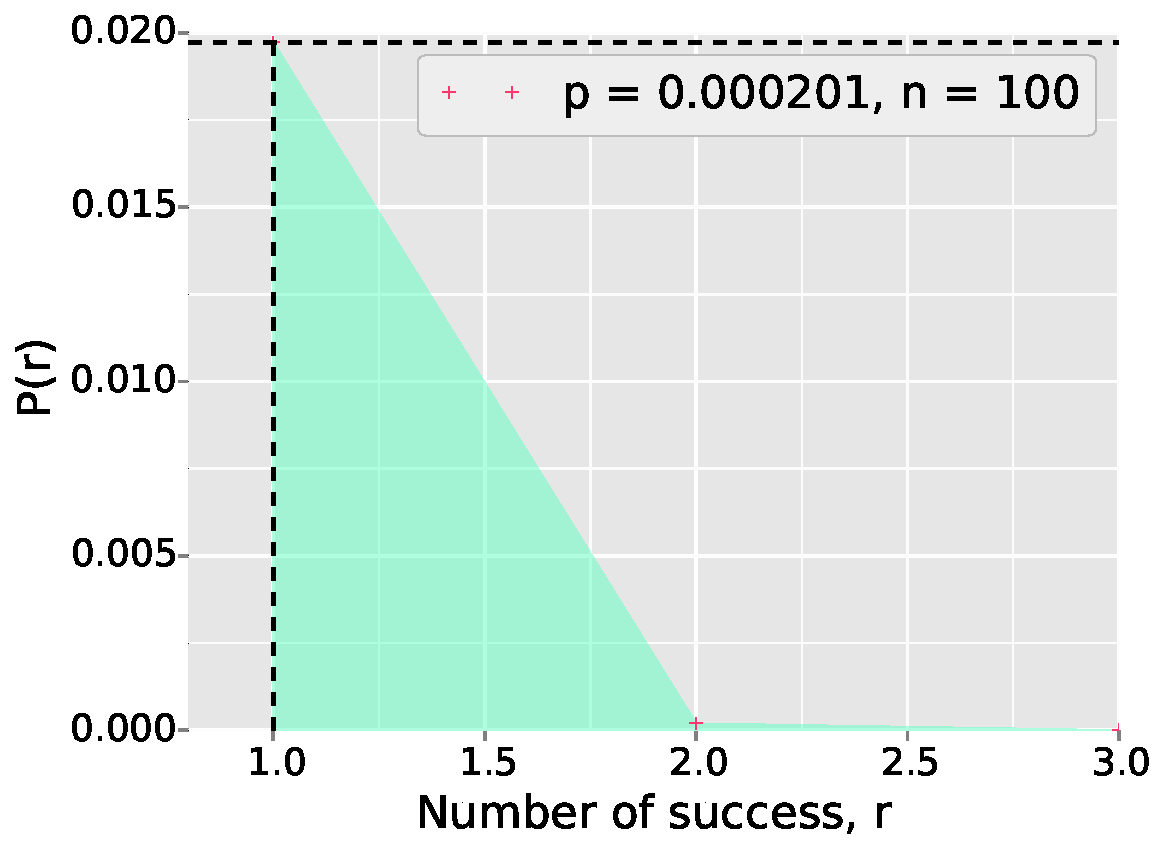
\includegraphics[width=.4\textwidth]{fig/lil_2.pdf}
		\end{center}
		\caption{Probability of getting out of 100 tries 18 successes out of 20 coin filps. The parameters are reported in the legend, and the shadowed area quantifies the chance of getting one or more times 18 successes.}
		\label{fig:lil2}
	\end{figure}
% subsection  (end)
% section Distributions and probabilities (end)
\section{Error propagation} % (fold)
\label{sec:error_propagation}
\subsection{}
Three different ways are employed to calculate the average of the given measurements, namely the arithmetic mean, a error weighted mean and finally a fit with a zeroth order polynomial.
The last two options require to accept and believe in the reported experimental errors.
The results are reported in Figure~\ref{fig:g}.
\begin{figure}[h!]
	\begin{center}
		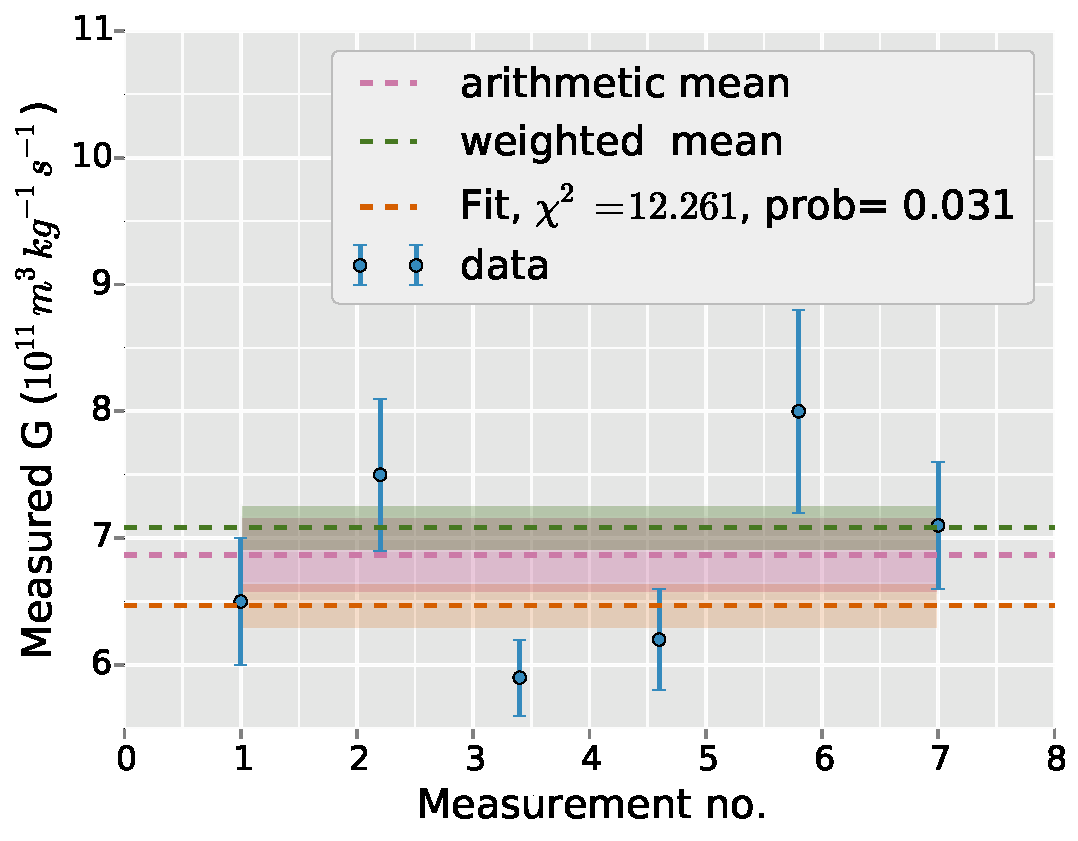
\includegraphics[width=.4\textwidth]{fig/g.pdf}
	\end{center}
	\caption{Graphical presentation of the given measurements and three differently calculated averages. The shadowed areas around each average value are $\pm \sigma_{\mu}$ the associated error.}
	\label{fig:g}
\end{figure}
The $\chi ^2 $ probability density function is reported in Figure~\ref{fig:xpdf} along with the probability of getting the same $\chi ^2 $ found in the aforementioned zeroth order polynomial fit.

\begin{figure}[!]
	\begin{center}
		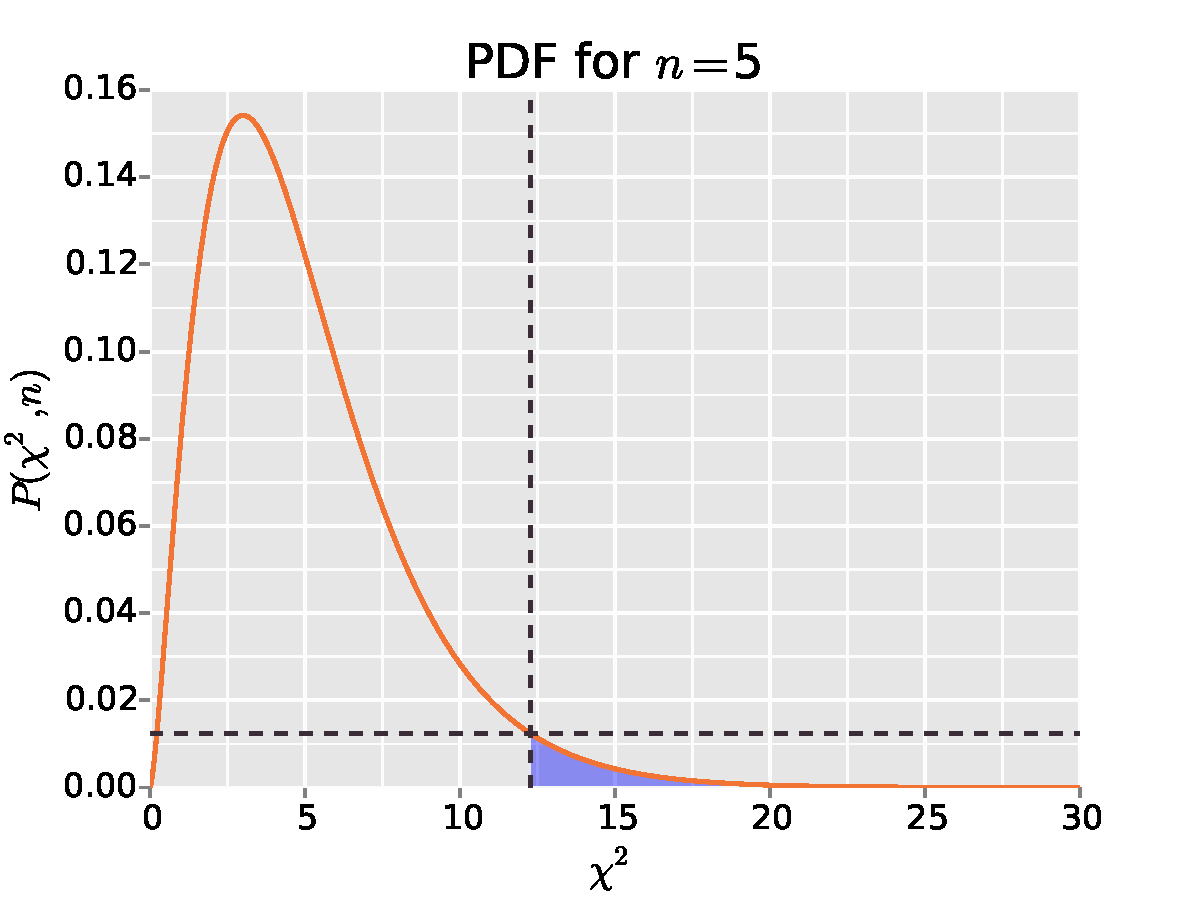
\includegraphics[width=.4 \textwidth]{fig/xpdf.pdf}
	\end{center}
	\caption{$\chi^2$ distribution for five degrees of freedom.}
	\label{fig:xpdf}
\end{figure}
% section error_propagation (end)

\clearpage
\section{Monte Carlo} % (fold)
\label{sec:monte_carlo}

% section monte_carlo (end)

\section{Statistical tests} % (fold)
\label{sec:statistical_tests}

% section statistical_tests (end)


\section{Fitting data} % (fold)
\label{sec:fitting_data}

% section fitting_data (end)
\end{document}